\documentclass{ctexart}

\usepackage{graphicx}

\title{流时代的答案 \\
       流数据库 HStreamDB 正式开源!}
\author{wangbin@emqx.io}
\date{\today}

\begin{document}
\maketitle

%% HStream 开创的流数据库,
%% 将成为未来企业软件系统的核心基础设施。
%%
%% 这篇文章的主题是介绍 HStreamDB 这个项目,
%% 要讲清楚:  
%% - 为什么要有这个项目?
%% - HStreamDB 是什么?
%% - 它解决了哪些问题?
%% - 它的功能特性有哪些?
%% - 它的使用场景有哪些? 
%% - 它如何使用?
%% - 它相比其它已有的方案有哪些优点? 
%% - 它目前的开发状态? 
%% - 它未来的发展规划? 
%% - 它的开源社区的情况? 
%% 
%% 标题:EMQ 全新流数据库项目 HStreamDB 正式开源!
%% 章节划分:
%% 1. HStreamDB 项目概述
%%    主要先讲项目的背景,也就是我们为什么要做这个项目,
%%    承接一下流数据库那篇,
%%    接着就引入到对项目本身的介绍,
%%    有一段话来介绍 hstreamdb 的项目定位,
%%    回答它是什么,解决什么问题。
%%    然后介绍一下它的整体架构。
%% 2. HStreamDB 架构和功能特性   
%% 3. HStreamDB 应用场景
%% 4. HStreamDB 快速上手
%% 5. HStreamDB 开源社区和发展规划
\section{HStreamDB 项目概述}

%% 背景(为什么要做?)
%% 流计算演进的背景,
%% 数据库发展的背景,
%% 物联网的背景,
%% 
%% 上一篇文章中我们跟大家介绍了流数据库这一全新的数据库品类,
%% 用来提供对流式数据的存储、处理、分析的一站式解决方案,
%% 相信大家对流数据库的概念有了基本的了解,
%% 今天这篇文章我们将向大家介绍我们目前正在研发的一款流数据库 HStreamDB.
%% 重申一下上一篇文章里面提到的关键观点:
%% - 新的数据存储和计算需求催生新的数据库品类。
%% - 流式数据做为一类新的数据类型,正在变得越来越流行,越来越重要。
%% - 当前还没有针对流式数据的数据库系统。
%% - 当前针对流式数据的解决方案存在着一系列的问题,
%%   根本问题是没有从全局的角度出发,给出一个系统的解决方案。
%% - 而流数据库是最终应有的解决方案。
%% - hstreamdb 就是这样一款流数据库。
%%
%% 直接引用上篇文章或许不太合适?
%% 这篇本身自己应该自包含才合适。
%% 
%% HStreamDB 是 EMQ 贯彻流数据库的理念,
%% 针对大规模实时数据流的接入、存储、处理、分发的
%% 全生命周期管理,
%% 使用标准 SQL (及其拓展)作为主要接口语言,
%% 以实时性作为主要特征,
%% 旨在简化数据流管理的流数据库。

上一篇文章[链接]中我们跟大家介绍了流数据库这一全新的数据库品类,
相信大家对流数据库的概念有了基本的了解,
今天这篇文章我们将向大家介绍我们目前正在研发的一款流数据库 HStreamDB.

HStreamDB 是一款专为流式数据设计的,
针对大规模实时数据流的接入、存储、处理、分发等环节进行全生命周期管理的流数据库。
它使用标准 SQL (及其流式拓展)作为主要接口语言,
以实时性作为主要特征,
旨在简化数据流的运维管理以及实时应用的开发。

%%HStreamDB 是一款专为 IoT 场景设计的, 
%%集大规模流式数据存储和实时流处理于一体的,
%%旨在简化流处理任务的开发和维护,
%%简化技术栈,
%%统一心智模型,
%%可扩展,
%%可以直接用 SQL 做流处理的,
%%流数据库。
%%促使用户能够对瞬变的数据做出快速响应,
%%从而交付更好的用户体验,
%%获取实时的数据洞察,
%%以及及时的商业决策。

HStreamDB 的整体架构如下图所示,
单个 HStreamDB 节点主要由 HStream Server (HServer) 和 HStream Storage (HStore) 两个核心部件组成,
一个 HStream 集群由若干个对等的 HStreamDB 节点组成,
客户端可连接至集群中任意一个 HStreamDB 节点,
并通过熟悉的 SQL 语言来完成各种从简单到复杂的流处理和分析任务。

\begin{figure}
  \centering
  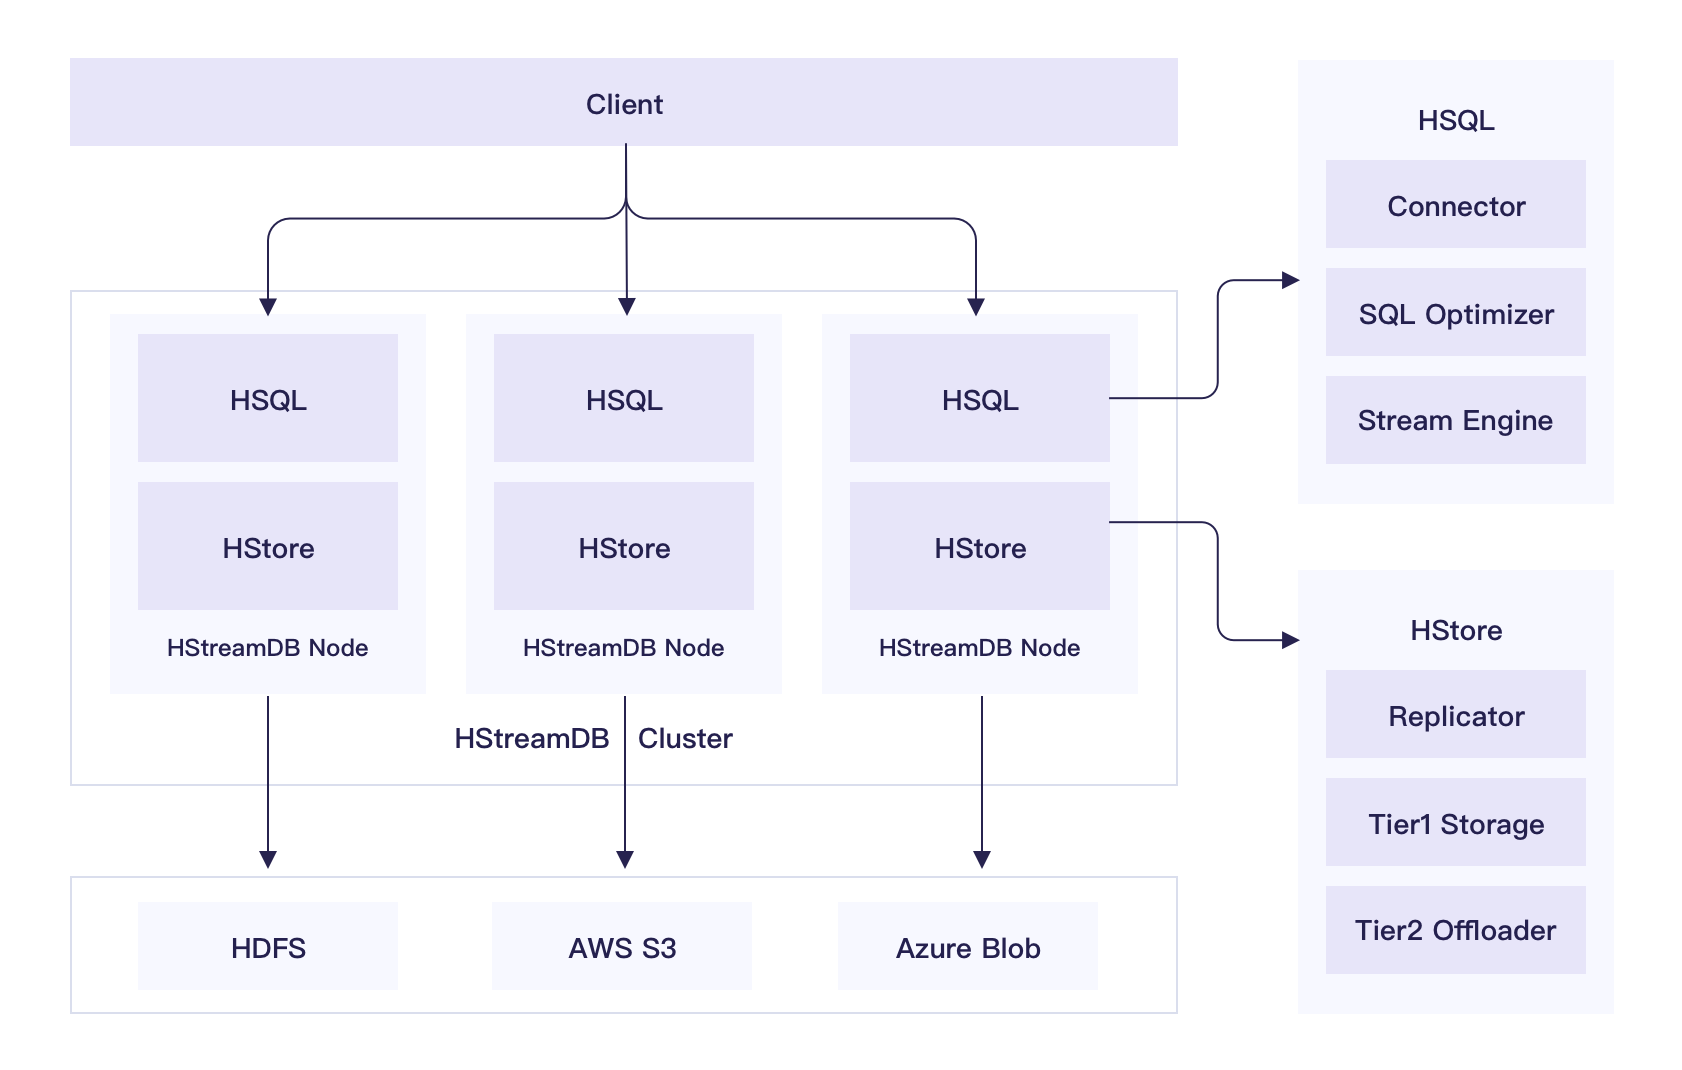
\includegraphics[width=\textwidth]{pic/hstream-arch.png}
  \caption{HStreamDB 整体架构}
  \label{fig:hstream-arch}
\end{figure}

HStream Server (HServer) 作为 HStreamDB 的核心计算组件,
其本身被设计为无状态的,
它主要负责客户端的连接管理,安全认证,
SQL 解析,SQL 优化,
以及流计算任务的创建、调度、执行和管理等。

具体的,HStream Server (HServer) 自顶向下可分为以下几层结构:
\begin{enumerate}
    \item 接入层。主要负责客户端请求的协议处理、
    连接管理、以及安全认证和访问控制。
    \item SQL 层。客户端主要通过 SQL 与 HStreamDB 交互,
      来完成大部分流处理和实时分析的任务。
      这一层主要负责将用户提交的 SQL 语句编译成数据流图
      传递给下一层继续处理。
      与经典的数据库系统一样,
      这里包含两个核心的子组件:SQL 解析器 和 SQL 优化器。
      SQL 解析器负责负责完成词法分析、语法分析,将 SQL 语句
      编译到对应的关系代数表达式;
      SQL 优化器与关系数据库主流的 CBO 优化器不同,
      除了负责基本的关系代数优化、基于规划的优化外,
      还有就是要做基于 streaming context 的特殊优化,
      比如 streaming fusion 之类的。
    \item Stream 层。
      这一层包含各种常见的流处理算子的实现,
      以及表达数据流图的数据结构和 DSL,
      还支持用户自定义函数作为处理算子。
      这一层主要负责为 SQL 层传递下来的逻辑数据流图
      选择对应的算子实现,生成可执行的数据流图。
    \item Runtime 层。
      这一层负责实际执行数据流图的计算任务并返回结果。
      主要包含任务调度器、状态管理器以及执行优化器等组件。
      其中调度器负责计算任务在可用计算资源之间的调度,
      可能是在单个处理的多线程之间调度,
      也可能是在单机的多处理器之间调度,
      或者是在分布式集群的多台机器或容器之间调度。
      状态管理器负责协调流出里算子的状态维护和容错。
      执行优化器可以通过自动化并行等手段加速数据流图的执行。
\end{enumerate}

HStream Storage (HStore) 作为 HStreamDB 的核心存储组件,
它是专门为流式数据设计的低延时存储组件,
不但能够分布式持久化存储大规模实时数据,
而且能够通过 Auto Tiring 机制,
无缝对接 S3 之类的大容量二级存储,
实现历史数据和实时数据的统一存储。

HStream Storage (HStore) 的核心存储模型是非常贴合流式数据的
日志模型,数据流本身可以看作是一个无限增长的日志,
它支持的典型操作包括追加写和区间读,
不支持任何更新和删除操作。

HStream Storage (HStore) 可分为以下几个层次:
\begin{enumerate}
    \item Streaming Data API 层。
       
      这一层提供核心的数据流管理和读写操作,
      包括数据流的创建、删除,
      以及向数据流中写入数据和消费数据流中的数据。
      在 HStore 对创建的数据流的数量没有限制,
      同时能支持大量数据流的并发写入,
      在大量数据流并发写入的时候依然能够保持稳定的低延迟,
      HStore 的存储设计中并没有按照数据流来做存储,
      因此数据流的创建是非常轻量的操作。
      针对数据流的特点,
      HStore 提供了 append 操作支持数据快速写入,
      同时在读取流数据方面,
      提供了基于订阅语义的 read 操作,
      数据流中新写入的数据会被迅速推送给消费者。

    \item 复制层(replicator)。
     这一层主要基于优化的 Paxos 共识引擎实现了流数据的强一致复制,
     保证数据的容错和可高可用性。

     通过非确定性放置的策略,
     最大化集群数据的均衡和可用性。

     支持复制组在线变配,
     在线水平扩展,
     数据均衡,
     自动伸缩。

     本层提供流数据存储的核心接口和实现,
     将连续的数据流统一抽象为基本的日志模型。
     内部的基本存储单元称为 segment,
     该层通过在各个存储节点间通过自动均衡 segment
     来实现存储层的水平扩展。
     写入的每份数据会复制到多个存储节点来保证可靠性
     和容错。
     该层还提供可选的数据索引支持,
     可为保存的数据生成索引,
     典型的包括主键(业务 key)索引和时间戳索引。
     该层还需要提供 compress 和 compact 支持。
    \item 一级存储层。
      本地存储基于 RocksDB 存储引擎,
      按时间片划分 column family 的方式,
      只使用 L0 的 SST Files,
      支持数据高速写入,

      最新写入的数据一般保存在磁盘上,
      或者通过存储节点内部的嵌入式数据库写入。
      由于磁盘存储成本较高,
      不适合将大量数据直接保存在磁盘上,
      支持通过配置自动将冷数据转储到更便宜的云存储上。
    \item 二级存储层。
        该层为多种长期存储系统提供统一的接口,
        支持诸如 HDFS, AWS S3 等,
        实现实时数据和历史数据的统一访问。
\end{enumerate}

\section{HStreamDB 功能特性}

\begin{figure}
  \centering
  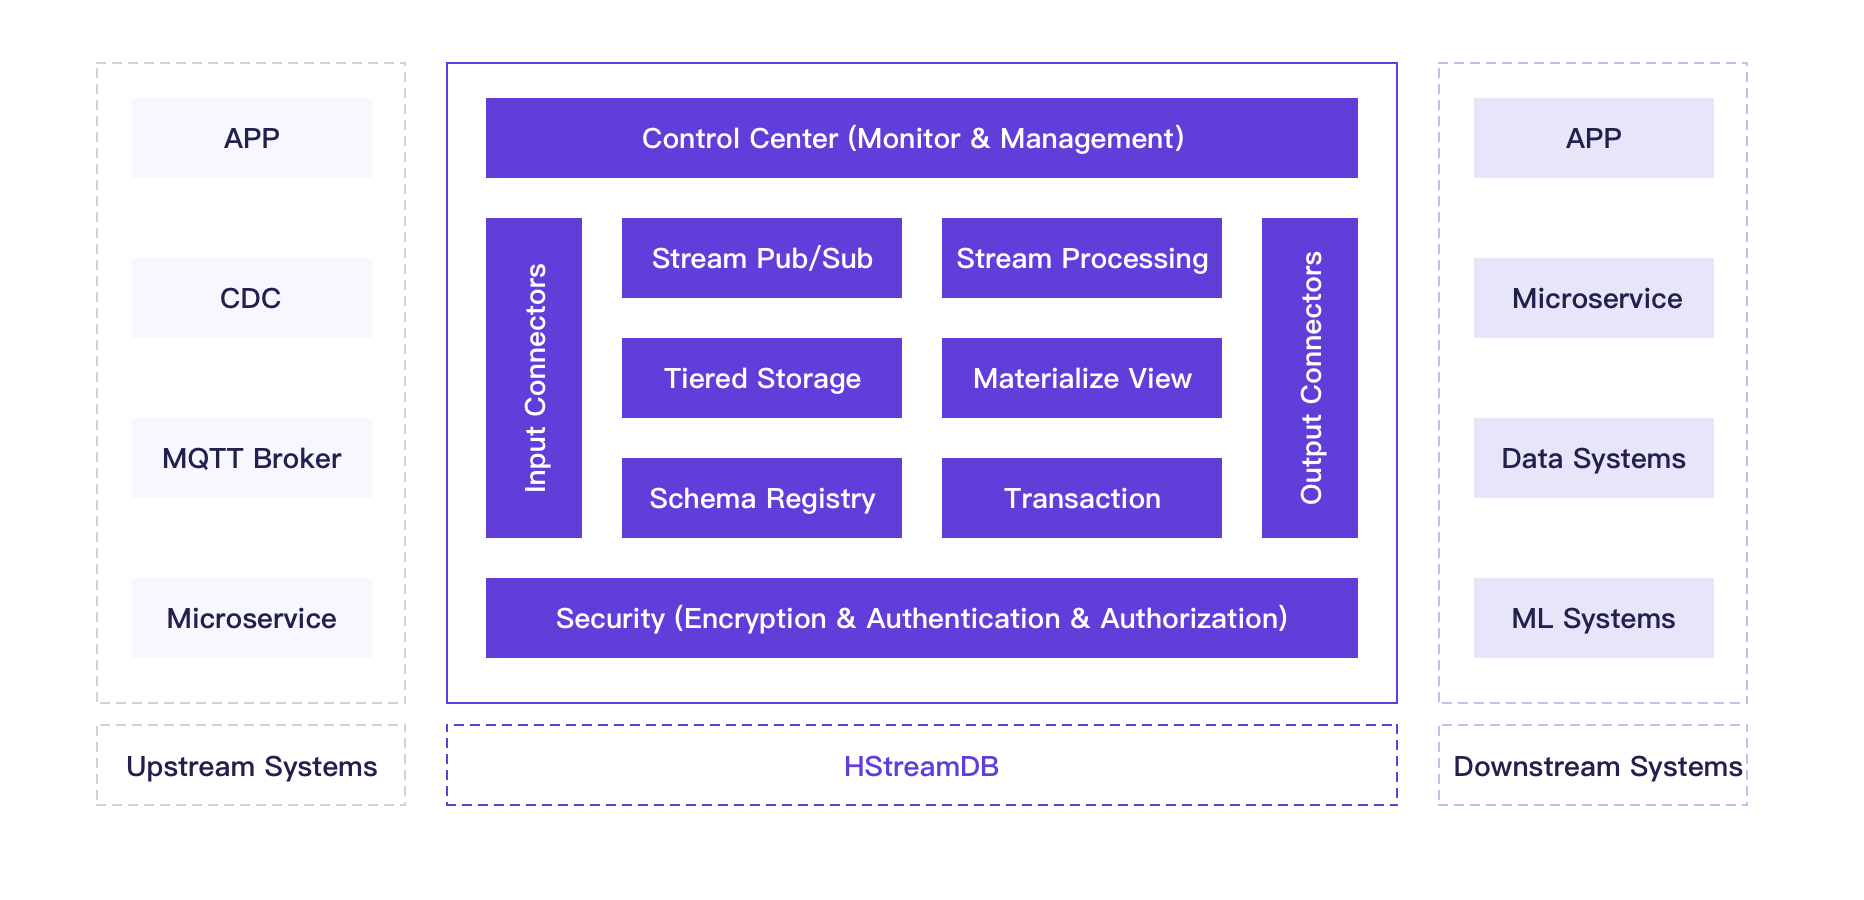
\includegraphics[width=\textwidth]{pic/hstream-features.png}
  \caption{HStreamDB 功能架构}
  \label{fig:hstream-features}
\end{figure}

\subsection{基于 SQL 的数据流处理}

HStreamDB 提供基于事件时间的完整的流处理能力,不仅支持基本的过滤、转
换操作,还支持按 key 做聚合计算,基于多种时间窗口的计算,以及数据流
之间 join 的能力,同时也支持乱序和晚到的消息的特殊处理,保证计算结
果的准确性。用户只需要通过 SQL 语句就能完成上述所有的处理功能,无
需学习任何三方 API。HStream 的流处理还提供了丰富的扩展能力,用户
可以针对自己的业务自行扩展。

\subsection{数据流的物化查询}

高效的增量计算引擎,timely flow,
支持快速的增量计算,
维护大规模物化视图的实时更新。

HStreamDB 提供了物化视图的功能,支持在持续更新的数据流上进行查询操
作。 HStream 内部会根据数据流的变化实时更新物化视图,用户可通过 SQL
语句查询物化视图获得实时的数据洞察。

\subsection{数据流管理}

支持创建大量的数据流,
在大量数据流并发写入的情况下仍然能够保持稳定的低延迟。

[TODO:修改]
方案基于经典的 Pub/Sub 模型,提供互斥订阅,共享订阅等多种订阅
模型,能够灵活应对不同的业务需求。同时 HStream 集群能够支持百万量
级的 Topic,在大量 Topic 数据写入的情况下依然能保证稳定的消费时延。

\subsection{数据流的持久化存储}

方案提供低延时的可靠的数据流存储,保证写入的数据消息不丢失,并
且能够重复消费。HStream 会将写入的数据消息复制到多个存储节点,提
供高可用和容错能力。HStream 同时支持将冷数据转储到成本更低的存储
服务上,比如对象存储,分布式文件存储等,存储的容量可无限扩展,能够
实现数据的永久存储。

\subsection{数据流的 Schema 管理}

HStreamDB 提供了内建的 Schema 管理功能,支持包括 Json, Avro, Protobuf 等
多种格式的 Schema 存储,同时也支持 Schema 的演化,管理多版本 Schema
之间的兼容性。通过 Schema 能够提升数据消息的质量,简化消费的流程,
避免很多不必要的数据错误。

\subsection{数据流的接入和分发}

HStreamDB 提供了和包括 MQTT Broker, MySQL,ElasticSearch, Redis 等多
种数据系统相连接的 Connector,方便用户和外部的数据系统进行集成。

\subsection{安全机制}

HStreamDB 提供包括 TLS 加密传输,基于 OAuth, JWT 等的身份认证以及授
权机制,同时预留了安全插件的接口,用户可根据需要对默认的安全机制进
行扩展。

\subsection{监控和运维工具}

HStreamDB 提供了基于 Web 的控制台,包含大量的系统仪表盘和可视化图表,
能够对集群机器状态,系统关键指标等进行详细的监控,方便运维人员对集
群进行管理。

\section{HStreamDB 应用场景}

\subsection{实时数据分析}

传统的数据分析通常基于批处理技术,
批处理一般是在预先收集好的有限的数据集上运行,
因此分析的结果往往不包含最新的数据,
有较高的时延。
HStreamDB 能够对实时的数据流进行分析,
并随着数据流的变化及时地更新结果,
这能够更好的支持诸如网站用户活动实时预测、
物联网传感器数据实时分析等应用。
相比批处理,
不但能提供更实时的数据洞察,
而且避免了周期性调度批处理任务的易出错和复杂性。

\subsection{事件驱动应用}

事件驱动应用通常是根据到来的事件实时触发对应的动作或行为,
它可以是无状态的或者带状态的,
比如:
金融交易中的实时欺诈检测,
业务流程监控预警,
物联网规则引擎等。
基于 HStreamDB,
实现这些复杂的事件驱动应用可能仅仅需要几条 SQL 语句,
大大降低了开发和维护这些应用的成本。

\subsection{实时数据管道}

企业内部往往需要在多个数据系统之间进行数据同步和迁移,
比如将在线的事务数据库中的数据拷贝到离线的数据仓库进行分析,
这个过程通常是由一套 ETL 系统完成的,
这类 ETL 系统的开发和维护成本都比较高,
而且它的数据同步往往不是实时的,
扩展性也比较差。
HStreamDB 集成了多种外部系统的连接器,
能够非常方便地搭建实时的数据管道,
实现实时构建索引,实时构建缓存等数据同步任务。

\subsection{在线机器学习}

如今机器学习系统在业务系统中起着越来越重要的作用,
包括搜索、推荐、风控等背后都广泛依赖机器学习系统。
然而随着在线业务及相关应用场景的井喷式发展,
常规的离线系统及离线机器学习平台已无法满足业务发展要求。
HStreamDB 的实时计算引擎能够助力机器学习系统的实时化,
实现在线特征提取,实时推荐等应用。

\section{HStreamDB 快速上手}

[copy from quickstart]


\section{HStreamDB 开源社区和发展规划}

[阐述我们对开源的信仰...]
EMQ 始终是一家开源的基础软件供应商,
我们坚信开源的价值与力量...

HStreamDB 从立项之初就完全采用开源的方式的进行开发,
目前项目还处在早期阶段,
我们诚邀各位感兴趣的开源社区的小伙伴们和我们一同开发。

目前 HStreamDB 的原型阶段开发完毕,
大家可以通过 Docker 安装并试用它的基本功能,
后续的分布式处理支持,
Schema 管理,
SQL 优化,
以及监控和运维等功能
能正在积极的陆续开发和完善中,
敬请期待!

\end{document}
